\documentclass[preview]{standalone}

\usepackage{amsmath}
\usepackage{amssymb}
\usepackage{bettelini}
\usepackage{stellar}
\usepackage{definitions}

\begin{document}

\id{measuretheory-lebesgue-spaces}
\genpage

\section{The Space L1}

\begin{snippet}{integral-norm-on-continuous-functions}
    The space \(\mathcal C^0([0,1])\) is Banach with the uniform norm. On the
    same vector space one may instead consider
    \[
        \|f\|_1=\int_0^1|f(x)|\,dx.
    \]
    Convergence for this norm means
    \[
        \int_0^1|f_n-f|\,dx\longrightarrow0,
    \]
    and has no direct implication of pointwise or uniform convergence. With
    this norm, \(\mathcal C^0([0,1])\) is not complete.
\end{snippet}

\begin{snippetexample}{continuous-functions-integral-norm-not-complete}{Continuous functions are not complete in the integral norm}
    For \(n\geq1\), define
    \[
        f_n(x)=
        \begin{cases}
            n & x\in[0,1/n^2],\\
            x^{-1/2} & x\in[1/n^2,1].
        \end{cases}
    \]
    \begin{center}
        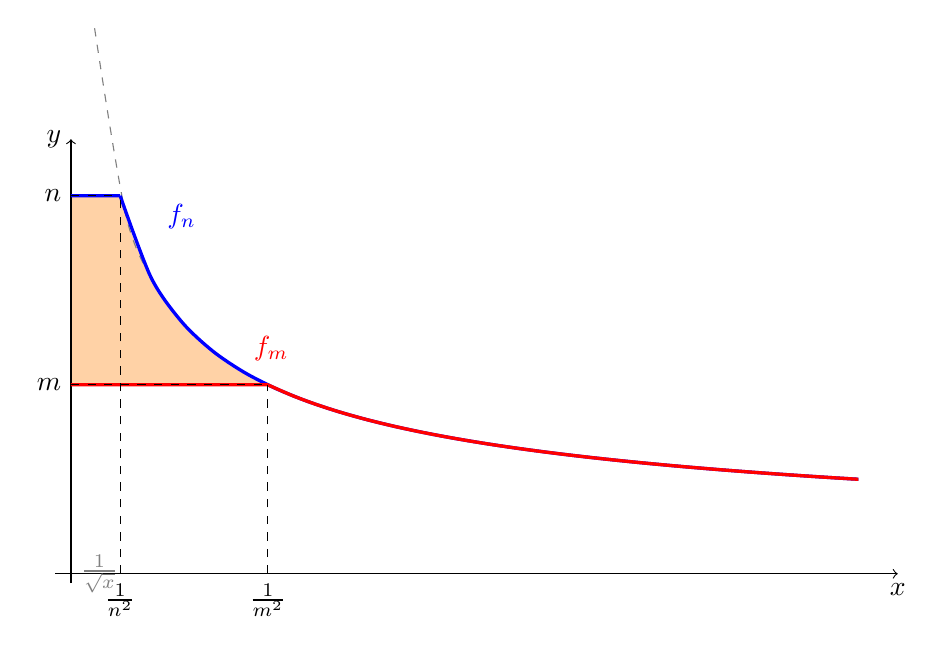
\begin{tikzpicture}[x=10cm,y=1.2cm]
            \def\m{2}
            \def\n{4}
            \pgfmathsetmacro{\xm}{1/(\m*\m)}
            \pgfmathsetmacro{\xn}{1/(\n*\n)}
            \pgfmathsetmacro{\xmax}{1.05}
            \pgfmathsetmacro{\ymax}{4.6}

            \fill[orange!35] (0,\m) rectangle (\xn,\n);
            \fill[orange!35] plot[domain=\xn:\xm,smooth] (\x,{1/sqrt(\x)}) -- (\xm,\m) -- (\xn,\m) -- cycle;

            \draw[->] (-0.02,0) -- (\xmax,0) node[below] {$x$};
            \draw[->] (0,-0.1) -- (0,\ymax) node[left] {$y$};

            \draw[dashed,gray] plot[domain=0.03:1,smooth] (\x,{1/sqrt(\x)}) node[pos=0.82,right] {$\frac{1}{\sqrt{x}}$};

            \draw[very thick,blue] (0,\n) -- (\xn,\n) plot[domain=\xn:1,smooth] (\x,{1/sqrt(\x)});
            \draw[very thick,red] (0,\m) -- (\xm,\m) plot[domain=\xm:1,smooth] (\x,{1/sqrt(\x)});

            \draw[dashed] (\xn,0) -- (\xn,\n);
            \draw[dashed] (\xm,0) -- (\xm,\m);
            \draw[dashed] (0,\n) -- (\xn,\n);
            \draw[dashed] (0,\m) -- (\xm,\m);

            \node[left] at (0,\n) {$n$};
            \node[left] at (0,\m) {$m$};
            \node[below] at (\xn,0) {$\frac{1}{n^2}$};
            \node[below] at (\xm,0) {$\frac{1}{m^2}$};

            \node[blue,above right] at (0.11,3.55) {$f_n$};
            \node[red,above right] at (0.22,2.15) {$f_m$};
        \end{tikzpicture}
    \end{center}
    If \(n>m\), then
    \begin{align*}
        \|f_n-f_m\|_1
        &=\int_0^{1/n^2}(n-m)\,dx
        +\int_{1/n^2}^{1/m^2}\left(\frac1{\sqrt x}-m\right)dx\\
        &=\frac1m-\frac1n\longrightarrow0.
    \end{align*}
    Thus \(\{f_n\}\) is Cauchy. On the other hand,
    \(f_n(x)\to x^{-1/2}\) for every \(x>0\), and
    \[
        \int_0^1\left|f_n(x)-\frac1{\sqrt x}\right|dx
        =\frac1n\longrightarrow0.
    \]
    The limit \(x^{-1/2}\) belongs to \(\mathcal L^1((0,1))\) but has no
    continuous representative on \([0,1]\). Therefore
    \((\mathcal C^0([0,1]),\|\cdot\|_1)\) is not complete.
\end{snippetexample}

\begin{snippet}{metric-completion-interpretation}
    A metric space can be completed by considering its Cauchy sequences and
    identifying two sequences \(\{x_n\}\) and \(\{y_n\}\) when
    \(d(x_n,y_n)\to0\). A convergent Cauchy sequence is equivalent to the
    constant sequence at its limit. The quotient fills precisely the missing
    limits. This motivates looking for the completion of
    \(\mathcal C^0([0,1])\) in the integral norm.
\end{snippet}

\begin{snippetdefinition}{integral-seminorm-definition}{Integral seminorm}
    Let \((X,\mathcal M,\mu)\) be a measure space. On
    \(\mathcal L^1(\mu)\), define
    \[
        \|f\|_1\triangleq\int_X|f|\,d\mu.
    \]
    This is a seminorm: it is nonnegative, positively homogeneous and
    subadditive, but \(\|f\|_1=0\) only implies that \(f=0\) almost
    everywhere, not necessarily everywhere.
\end{snippetdefinition}

\begin{snippetdefinition}{l-one-space-definition}{The space \(L^1\)}
    Let
    \[
        N=\{f\in\mathcal L^1(\mu)\suchthat f=0\text{ almost everywhere}\}.
    \]
    The space \(N\) is a vector subspace of \(\mathcal L^1(\mu)\). Define
    \[
        L^1(\mu)\triangleq\mathcal L^1(\mu)/N.
    \]
    Its elements are equivalence classes of integrable functions under
    equality almost everywhere.
\end{snippetdefinition}

\begin{snippetproposition}{integral-seminorm-descends-to-l-one-norm}{The integral seminorm defines a norm on \(L^1\)}
    The expression
    \[
        \|[f]\|_1=\int_X|f|\,d\mu
    \]
    is well-defined on \(L^1(\mu)\) and is a norm.
\end{snippetproposition}

\begin{snippetproof}{integral-seminorm-descends-to-l-one-norm-proof}{integral-seminorm-descends-to-l-one-norm}{The integral seminorm defines a norm on \(L^1\)}
    If \(f=g\) almost everywhere, then \(|f|=|g|\) almost everywhere, so
    \[
        \int_X|f|\,d\mu=\int_X|g|\,d\mu.
    \]
    Thus the expression is independent of the representative. Homogeneity
    and the triangle inequality descend from \(\mathcal L^1\). Finally,
    \(\|[f]\|_1=0\) implies \(f=0\) almost everywhere, hence
    \([f]=[0]\).
\end{snippetproof}

\end{document}
